\documentclass[11pt]{article}
\usepackage{icmlko}
\begin{document}

\title{목록이 정렬돼 있으면 표본을 늘려도 늘어난 쪽이 다른 모집단이다}
\author{월드모델 실험실}
\date{노트 374 · 2026년 8월 1일}
\maketitle

\begin{abstract}
노트 373이 ``이제 남은 것은 수집뿐''이라 적고 펀딩을 \emph{버림 0\% ---
이미 다 쓴다}로 분류했다. \textbf{틀렸다.} 축이 레코드를 100\% 쓰는 것은
맞지만 \textbf{레코드가 77,515건 중 400건}이다. 늘리러 갔다가 더 큰 것이
나왔다.

\textbf{텀블벅 목록은 인기순으로 정렬돼 있다.} 캐시된 3,875쪽에서 쪽
번호와 라벨(log10 후원자)의 순위 상관이 $\mathbf{-0.3666}$ 이다(쪽
50\textasciitilde{}161 중앙 2.56 대 531\textasciitilde{}753 중앙 1.93).
우리 400건은 쪽 50\textasciitilde{}753 --- \textbf{위에서 19\%} 에서 왔다.
그래서 표본을 늘리면 늘어난 쪽이 체계적으로 다른 모집단이 된다: 옛 400 대
새 180 의 라벨 중앙이 $2.14$ 대 $2.46$, 맨휘트니 $p=1.5\times10^{-13}$.

\textbf{그리고 내 대표성 검사가 두 번 다 통과했다} --- 연도 분포로만 봤기
때문이다(2025+ 비율 20\% 대 19\%). 섞은 유보로 재면 펀딩이
$0.4195 \to 0.6019$ 로 뛰는데, 무리 안에서 다시 순위를 매기면
$\mathbf{+0.4385}$ 다. \textbf{0.16 이 표집 구조였다.}

수집 정렬이 과제를 정한 \textbf{네 번째} 도메인이다(도서 베스트셀러 ·
모바일 인기 차트 · 만화 인기순 · 펀딩). 고침은 싸다 --- 목록 전체가 이미
캐시에 있다(자격 있는 것 \textbf{75,434건}, 그중 2025년 이후
\textbf{13,030건}). 균일 무작위 표집기를 만들어 돌리는 중이다.
\end{abstract}

\section{노트 373을 정정한다}

노트 373이 펀딩을 이렇게 적었다: \emph{레코드 400 $=$ 축 400, 버림 0\%.
유보 80은 2025+ 가 그만큼뿐 $\to$ 새 수집만.} 앞은 맞고 \textbf{뒤가
틀렸다} --- ``2025+ 가 80건뿐''은 세계에 대한 사실이 아니라
\texttt{--want 400} 에서 멈춘 결과다. 목록에는 77,515건이 있다.

\section{목록이 정렬돼 있다}

\begin{center}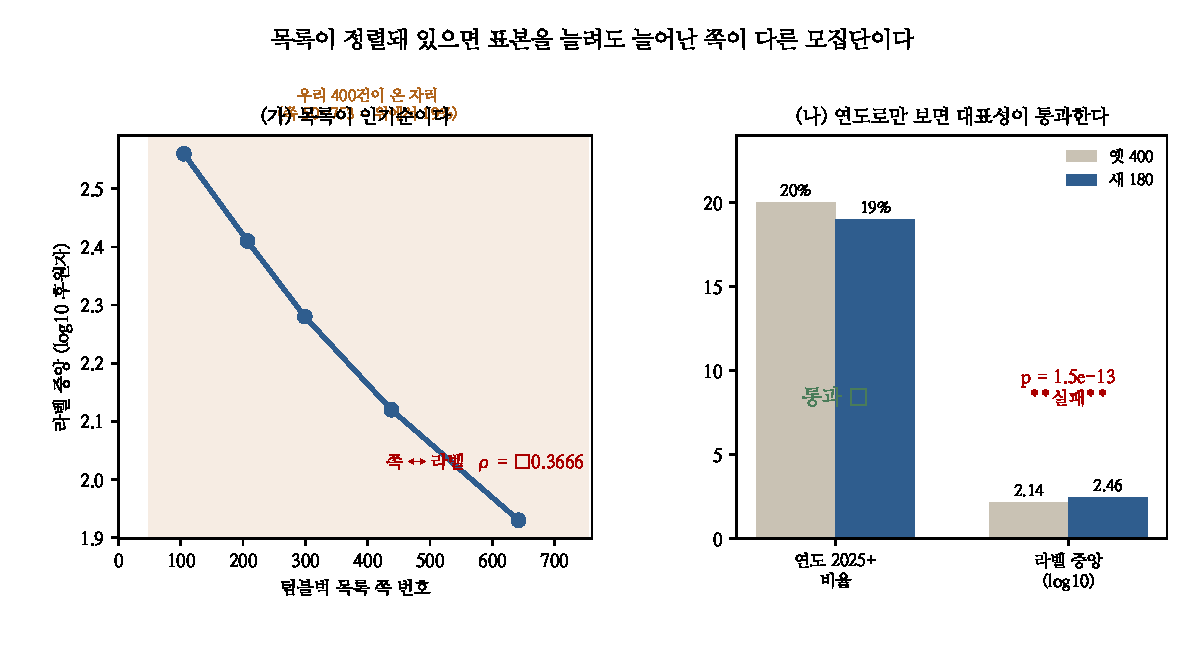
\includegraphics[width=\linewidth]{figs/sorted.pdf}\end{center}

캐시된 목록 3,875쪽 · 77,495건에서 각 레코드의 출처 쪽을 붙여 봤다.

\begin{center}
\begin{tabular}{lrr}
\hline
쪽 구간 & $n$ & 라벨 중앙 \\
\hline
50\textasciitilde{}161 & 140 & 2.56 \\
161\textasciitilde{}253 & 140 & 2.41 \\
253\textasciitilde{}346 & 140 & 2.28 \\
346\textasciitilde{}531 & 130 & 2.12 \\
531\textasciitilde{}753 & 140 & 1.93 \\
\hline
\multicolumn{3}{c}{쪽 $\leftrightarrow$ 라벨 순위 상관 $\mathbf{-0.3666}$} \\
\hline
\end{tabular}
\end{center}

\texttt{funding\_domain.run} 은 \texttt{range(50, 3876, stride)} 를 돌면서
후보가 차면 멈춘다. \texttt{--want 400} 이면 스물몇 쪽에서 멈추므로
\textbf{목록 맨 위 19\%만 본다.}

\textbf{보폭을 바꿔도 안 고쳐진다.} 처음엔 ``보폭 7이라 앞쪽만 봤다''로
읽고 보폭을 자동 조정하게 고쳤는데, 다시 받은 180건도 라벨 중앙 2.46 에
$p=1.5\times10^{-13}$ 이었다. \emph{어느 보폭이든 앞에서부터 채우면 같다.}

\section{연도 검사는 통과하고 라벨 검사는 실패한다}

사전 등록에 대표성 확인을 적어 뒀다 --- \emph{새로 받은 것의 연도 분포가
기존과 비슷한지 먼저 본다.} 통과했다(2025+ 비율 20\% 대 19\%, 두 번 다).
\textbf{그런데 라벨이 갈렸다.}

\begin{center}
\begin{tabular}{lrrl}
\hline
 & 옛 400 & 새 180 & \\
\hline
2025+ 비율 & 20\% & 19\% & 통과 \\
라벨 중앙(log10 후원자) & 2.14 & 2.46 & $p=1.5\times10^{-13}$ \textbf{실패} \\
사분위 & $[1.83,\,2.50]$ & $[2.24,\,2.73]$ & \\
\hline
\end{tabular}
\end{center}

\textbf{규약: 표본을 늘렸으면 \emph{라벨} 분포를 견준다.} 연도는 정렬과
무관할 수 있고, 실제로 여기서는 무관했다.

\section{섞으면 점수가 부풀려진다}

두 무리를 한 유보에 넣고 재면 펀딩이 $0.4195 \to 0.6019$ 로 뛴다. 갈라
보면:

\begin{center}
\begin{tabular}{lrrl}
\hline
유보 부분집합 & $n$ & $\rho$ & 95\% 구간 \\
\hline
옛 80행 & 80 & $+0.4513$ & $[0.241,\,0.636]$ \\
새 105행 & 105 & $+0.4281$ & $[0.247,\,0.581]$ \\
\textbf{전부 185행} & 185 & $\mathbf{+0.5988}$ & $[0.487,\,0.696]$ \\
\hline
\multicolumn{2}{l}{무리 안에서 다시 순위} & $\mathbf{+0.4385}$ & \\
\hline
\end{tabular}
\end{center}

\textbf{전체가 두 부분집합 어느 쪽보다도 높다.} 라벨 중앙이 1.95 대 2.46,
예측 중앙이 236.8 대 570.2 로 \emph{같은 방향}이라 모형이 두 무리를 옳게
갈라 놓고, 그 무리 사이 순위가 $\rho$ 에 얹힌다. \textbf{0.16 이 표집
구조다.}

\textbf{노트 353 · 357 · 372와 같은 집안이고 부호가 반대다.} 거기서는
두 모집단이 섞여 $\rho$ 를 \emph{무너뜨렸고}, 여기서는 \emph{부풀린다}.
\textbf{두 모집단이 섞이면 점수는 어느 쪽으로든 움직인다 --- 낮아지는
것만 의심하면 안 된다.}

\section{고침은 싸다}

목록 전체가 이미 캐시에 있다 --- 3,875쪽 · 77,495건 · 자격 있는 것
\textbf{75,434건}(97\%)이고 그중 2025년 이후가 \textbf{13,030건}이다.
목록 호출 없이 균일 무작위로 뽑아 리워드만 받으면 된다.
\texttt{ingest/funding\_sample.py} 를 만들어 씨앗을 박고(노트 367의 재현
조항) 돌리고 있다. 지금까지 받은 것은 쪽 474\textasciitilde{}2974(중앙
1814)에 퍼져 있다 --- 옛 400의 50\textasciitilde{}753 과 다르다.

\textbf{챔피언은 안 건드렸다.} 균일 표본은 \texttt{funding\_uniform.json}
에 따로 쌓고, 다 모인 뒤 짝으로 재고 바꾼다.

\section{규약에 더하는 줄}

\begin{itemize}
\item \textbf{목록을 앞에서부터 채우지 마라.} 정렬돼 있으면 표본이
한쪽이 된다. 무작위로 뽑거나 전 구간을 훑는다.
\item \textbf{대표성은 라벨로 확인한다.} 연도 · 분야는 정렬과 무관할 수
있다 --- 여기서 두 번 다 통과했다.
\item \textbf{두 모집단이 섞이면 점수가 오를 수도 있다}(353 · 357 · 372는
내려갔고 여기는 올라간다). \emph{오르는 것도 의심한다.}
\item \textbf{``버림 0\%''는 다 썼다는 뜻이 아니다} --- 무엇을 못 모았는지는
안 나온다.
\end{itemize}

\section{남은 것}

\begin{center}
\begin{tabular}{ll}
\hline
갈래 & 지금 아는 것 \\
\hline
\textbf{균일 펀딩 2,500건} & 돌고 있다. 다 모이면 짝으로 재고 바꾼다 \\
다른 세 도메인의 정렬 & 도서 베스트셀러 · 모바일 인기 차트 · 만화 \\
 & 인기순. 같은 검사를 각각 돌린다 \\
팝업 실측 41행 & 노트 360 · 364 · 366 \\
\hline
\end{tabular}
\end{center}

둘째 줄이 이 노트가 여는 것이다 --- 정렬 편향이 네 도메인에서 확인됐으니,
\textbf{각 도메인의 라벨이 수집 순서와 얼마나 상관되는지}를 한 번에 재는
것이 다음이다.

\end{document}
